\chapter{级联传感器}
\label{chap-cassys}

本章介绍了创建传感器和通过自然语言的新工作方式的级联能力的工具\textit{Cassys} 
 \textit{传感器级联} \index{传感器级联}
一个应用于多个图形 (自动机和传感器), 表示于下列文字: 每个图形改变文本,并且可以通过下面的图可以用于进一步处理的变化。这种类型的系统主要用于解析,分块,信息提取,识别实体的命名等要做到这一点,CASSYs采用了一系列的“定位模式”用适当的选项。

\bigskip
\noindent \textit{CasSys} \index{CasSys}系统的第一个原型于2002年在实验室LI创建(Laboratoire d'Informatique de l'Université de Tours) (\cite{these-nathalie}). 
这个原型是完全致力于命名实体的抽取。然后CasSys推广到适用于任何类型,它需要一个级联更新。它多年来不断完善,实际上并没有在Unitex正在建设中。它是通过最近的一个项目\footnote{"Feder-Région 中心和实体的命名和可命名" 由Denis Maurel, LI, Tours, France完成,最终被Nathalie Friburger和David Nott实现},从而达到CasSys和Unitex的全面整合。

Unitex的语法是类型语境的自由并把有限状态自动机的结果转导领域的概念。用转换(转换器)的文法能够产生输出。 CASsys专门从事传感器在级联的形式应用。

\bigskip
级联可用于解析,分块,信息提取等。
\noindent因为它们允许给处于与输出图形识别的序列信息组合换能器是有趣。
这些输出可能是:
\begin{itemize}
\item被添加到所识别的序列,并显示在所得到的协议或经修正的文本。
\item更换公认的文本序列。
\end{itemize}
\noindent这两种操作变换文字或添加信息。

\bigskip
\noindent在本章中,我们将介绍如何创建级联传感器以及如何应用。然后,我们显示的选项,并提供CASSYs可能性。

%%%%%%%%%%%%%%%%%%%%%%%%%%%%%%%%%%%%%%%%%%%%%%%%%%%%%%%%%%%%%
\section{应用CASSYs级联传感器}
\label{section:applyCascade}
应用与Cassys转换级联是代表一种语言现象与换能器的列表,以适用于特定的顺序文本:CASSYs及其在Unitex接口可以实现它。本节将介绍如何使用界面来创建和管理的图(顺序,添加,删除),并应用了级联。 

%%%%%%%%%%%%
\subsection{创建传感器的列表}
\label{subsec:listTrans}

\bigskip
\noindent要管理传感器的列表中,FS表的菜单有两个子菜单:"\textit{新级联}" 和 "\textit{编辑级联……}" (Figure \ref{fig13-08}).要创建换能器的列表中,选择 "\textit{新级联}"。如果你想改变现有的级联关系,选择"\textit{编辑级联……}",然后选择新级联的关系。

\begin{figure}[!htb]
 \centering
 \includegraphics[width=4cm]{resources/img/fig13-08.png}
 \caption{Unitex中“FS表”的子菜单下的"新级联"和"\textit{编辑级联……}"}
 \label{fig13-08}
\end{figure}

当前语言的目录包含子目录名为CasSYs其中级联配置文件的位置。这些是扩展名为\textit{.csc}是文本文件 (例如: ma cascade.csc)

\subsection{编辑传感器列表}
\label{subsec:editlistTrans}

CasSys的配置窗口 (\ref{fig13-03})有三个部分:

\begin{figure}[!htb]
  \centering
  \includegraphics[width=16cm]{resources/img/fig13-03.png}
  \caption{与换能器的右侧列表的Cassys配置窗口}
  \label{fig13-03}
\end{figure}

\begin{enumerate}
	\item 左侧的\textit{管理文件}留下的框架,您可以选择换能器放在级联。经理仅显示FST2文件(在列表中希望所有的图表必须编译FST2格式)。要编辑的级联,选择左边的图形和使用拖放把正确的。	
	\item  \textit{tableau}的右侧显示级联:选择每个图形传感器和选项的有序列表。该表显然是空的一个新的级联。		 
		表中的列 (Figure \ref{fig13-09})给每个图形的数量,并允许选择他们的行为。
	\begin{itemize}
	\item \textbf{\#} : 在级联的每个图表或转换器的编号;
 FST2的文件是编号。
	\item \textbf{禁用} : 要选择当前图形。 \textit{禁用} 表示: "\textit{不应用于级联}".
		未选中的图形出现没有编号,灰色和划掉。	\item \textbf{名称} : 图的名称(以 \emph{fst2}为拓展名). 如果你把鼠标放在图形的名称,工具提示出现带有图形的完整路径。这些图表,它的源文件不会出现斜体和红色。

	\item \textbf{整合}:如果换能器是在合并模式被应用。
	\item \textbf{替换}:如果换能器将被应用于在替换模式。
	\item \textbf{直到断点}:如果换能器是直到即达到一个固定点的文本是不变,以应用一次或数次(见\ref{sub:AppWhiCon})。
	\end{itemize}
	
	 \item该中心有以下说明的按钮:
		\begin{itemize}
		\item \textit{"上移一层"/"下移一层"/"置于顶层"/"置于底层"}用于改变在列表中换能器的顺序(它们移动选定的换能器); 
		\textit{"上移一层"} et \textit{"下移一层"}移动传感器选定行向上或向下, \textit{"置于顶层"} et \textit{"置于底层"}定位开始或列表的末尾。
		\item \textit{"删除"}将删除传感器的列表中选定的传感器。
		\item \textit{"添加"}在列表中增加一个换能器(预先选择的)。它将替代之前的。
		\item \textit{"视图"}打开两个在换能器的列表的文件浏览器中选择的曲线图。这是非常有用的快速访问任何转换器,以及采取一看,要改变。
		\item \textit{"保存"} 和 \textit{"另存为"}可以记录换能器的列表。缺省情况下,列出了换能器被放置在当前CASSYs语言的目录(例如法语/Cassys).
		\item \textit{"编辑"}编译级联的所有图形。	
		\item \textit{"禁用所有"}禁用级联的所有图形。	
		\item \textit{"启用所有"}选择级联的所有图形。	
		\item \textit{"关闭"}关闭当前窗口。
		\end{itemize}
\end{enumerate}


\begin{figure}[!htb]
  \centering
  \includegraphics[width=7cm]{resources/img/fig13-09.png}
  \caption{转译列表}
  \label{fig13-09}
\end{figure}

	

\subsection{引用级联}
\label{subsec:launchCascade}

在“文字”菜单中,选择子菜单"\textit{Apply CasSys cascade...}" (图\ref{fig13-01})打开窗口Cassys。此菜单"\textit{Apply CasSys cascade...}" 没被激活只有当文本之前已经被打开。
\begin{figure}[!htb]
 \centering
 \includegraphics[width=5cm]{resources/img/fig13-01.png}
 \caption{Unitex“文本”菜单下菜单和"引用CasSys级联"的子菜单}
 \label{fig13-01}
\end{figure}

CasSys窗口 (\ref{fig13-02})显示当前语言的CASSYs目录的内容。它可以让你选择包含传感器列表适用于文本文件。一旦选择了这个列表,你可以点击“启动”按钮应用级联。

\begin{figure}[!htb]
  \centering
  \includegraphics[width=10cm]{resources/img/fig13-02.png}
  \caption{打开级联传感器后的窗口}
  \label{fig13-02}
\end{figure}

在首选项中规定的形态方法的任何字典是你的图表可用。
首选项可以从菜单"Info" (Info -->Preferences --> morphological-mode dictionaries) 进行更改。

\subsection{共享级联传感器列表文件}
\label{subsec:shareCascade}

为了便于与CASSYs协同工作,一个输出/输入功能的设置有一个换能器列表文件。这种可能性是由菜单提供"\textit{文本 / 应用CasSys级联..}" (图 \ref{fig13-02}).

要共享一个级联列表文件,下面必须满足:
\begin{enumerate}
\item \textbf{Export :} 选择一个级联文件并单击“导出”按钮。 (可共享的文件在\texttt{/Cassys/Share})
\item将文件发送到共享你的同事\item \textbf{导入:} 选择文件并单击“导入”。
(准备的文件中使用的目录\texttt{/Cassys}中创建)
\end{enumerate}

%%%%%%%%%%%%%%%%%%%%%%%%%%%%%%%%%%%%%%%%%%%%%%%%%%%%%%%
\section{CasSys详细说明}

在本节中,我们提出了如何CASSYs的详细说明。

\subsection{使用的图表的类型}
\label{graphs-for-cassys}

CASSYs使用图形的编译版本(格式\verb+.fst2+). CASSYs管理本地语法(section~\ref{syntactic-graphs})在第\ref{chap-advanced-grammars}章介绍。
级联使用的语法遵循相同的规则,在国联语法常用。它们可以具有子图,使用形态学方法和形态滤波器,并参考信息中的字典。

\bigskip
\noindent CasSys不在\verb+fst2+兼容(\ref{section-debug-mode}).当与菜单\verb+Text> Locate Pattern+施加图形调试模式下,系统编译在调试模式下的特殊格式的曲线图。对于\verb+fst2+正常格式的文件,重建图,或者在菜单\verb+FSGraph+无论是在命令行或应用的图形与\verb+Locate Pattern+之前检查调试模式。

\subsection{使用迭代器}
\label{sub:AppWhiCon}

CASSYs可以在文本应用图形反复,直到获得新的匹配。这种行为是根据直到修复项目检查或没有\verb+Until fix point+每个图形。本节介绍了此选项的行为。

例如,考虑该图\ref{fig:AB->A}其中确认\emph{AB} 是本 \emph{A}替换。

\begin{figure}[!htbp]
  \centering
  \includegraphics[width=6cm]{resources/img/AB_to_A.png}
  \caption{转移器把A换成BA}
  \label{fig:AB->A}
\end{figure}

考虑文本 \emph{B B B A A A}。这段文字 \ref{fig:AB->A} 用了\emph{Until fix point}  : \\

\begin{tabular}{|l|cccccc|r|}
\hline
initial text  &B&B&B&A&A&A&\\
\hline
迭代1 & &B&B&A&A&A& 1 匹配\\
迭代2 & & &B&A&A&A& 1匹配\\
迭代3 & & & &A&A&A& 1匹配\\
迭代4 & & & &A&A&A& 0匹配\\
\hline
\end{tabular}

\bigskip
在前三次迭代中,获得一个匹配,图形,然后再次施加到得到的文本。在第四次迭代,没有找到匹配的,序列不再重新应用。
\bigskip
\large{\textbf{注意:}} 留意使用此选项可能关闭。例如,如果施加在实施例的文字识别\ EMPH{A}和\ EMPH{A}替换它的换能器会导致堵塞。


\subsection{XML语言的词汇标记}

作为输出,与词汇标签格式被转换成XML格式。
这种变化是为了提供更可操纵文本到终端用户所作出的。

从这种格式,它是比较容易得到的自适应输出在所有。\\

这些词汇标签更为确切 :\\
\begin{tabular}{c}
\texttt{
\{forme.lemme,code1+code2:flex1:flex2\}}
\end{tabular}\\

以下是Cassys输出XML的格式 :\\
\begin{tabular}{ll}
\texttt{<csc>}&\\
	&\texttt{<form>forme</form>}\\
	&\texttt{<lem>lemme</lem>}\\
	&\texttt{<code>code1</code>}\\
	&\texttt{<code>code2</code>}\\
	&\texttt{<inflect>flex1</inflect>}\\
	&\texttt{<inflect>flex2</inflect>}\\
\texttt{</csc>}&\\
\end{tabular}


\subsection{级联规则}

在级联中,Unitex每个图形中使用的规则如下:
\begin{itemize}
	\item插入左认可的原因:在“合并”模式,输出所插入的识别序列的左边。	\item	优先在最左边的理由:当地语法的应用过程中,重叠的事件都编入索引。在相关的结构中,所有这些实例都存在,但作为CASSYs修改级联的每个图形的应用后的文字,它是必要的,这些事件中进行选择所考虑的之一。优先考虑的是最左边的序列。
	\item优先较长的模式:在CASSYs,在图的应用是保守的最长序列。
	\item限制出现的次数流行:在CASSYs,这个数量不局限于:这样的限制在CASSYs没有意义。所有的事件总是在文本索引。
\end{itemize}

\subsection{CasSys的标记图谱}

输出换能器可以用来将信息插入文本,尤其是标记的识别理由:它可以使用)的任何种类的标记,((), [],'“等等。或XML标签,如<XXX> </ XXX>,但CASSYs提供注释认可的场地,提供我们现在提出了一些机会,一种特殊的方式。 

\bigskip
\noindent切割在不同类型的令牌的文本作为句子{S}的端部的标记; {STOP}标记,相邻字母序列,词汇标签{今天.ADV}等。词汇标签中使用CASSYs特别。词法标签(括号),通常被用来避免歧义(详见第\ref{tokenization}和\ref{section-displaying-sentence-automata}部分)。
例如,在一个字,如果你有令牌\emph{\{curly brackets,.N\}},即“大”或“括号”被识别,但只有整个序列“大括号”。词法标签可以包含一个复杂的词汇信息\emph{N+Pers+Hum:fs}。
在图中,有可能在一个词汇面具使用的信息找到一个令牌:\emph{<.N>}例如,我们可以写\ EMPH寻找一个名字,\emph{<.Pers+Hum>}这些词汇面具“搜索正则表达式”部分中描述\ref{section-special-symbols}.
 
\bigskip
\noindent 在CASSYs我们使用的词汇品牌特别。换能器级联有趣的是,找到一个岛上。有必要对这种类型的系统,以避免以前识别图案是不明确的与那些由下列图表识别。为了避免这种情况,我们的标签通过图表的形式确认的理由\emph{\{} 和\emph{,.tag1+tag2+tagn\}} (或 \emph{tag1, tag2, etc.} 是自己的标签).

\bigskip
\noindent为了解释这种现象,这里有一个简单的例子。这里我们正在努力的文字是:

\emph{bac a b c cc a b b ba ab a b bca a b c abaabc}.

\bigskip
\noindent 图grfAB (\ref{fig13-05})识别文本序列\emph{ab}并增加了词汇标签 \{a b,.AB\}.在合并模式应用于此图形添加 ajoute \emph{\{ } 和 \emph{,.AB\}} 
\begin{figure}[!htb]
  \centering
  \includegraphics[width=6cm]{resources/img/fig13-05.png}
  \caption{Le graphe grfAB}
  \label{fig13-05}
\end{figure}

\bigskip
\noindent由此产生的文字是: \emph{bac \{a b,.AB\} c cc \{a b,.AB\} b ba ab \{a b,.AB\} bca \{a b,.AB\} c abaabc}.

\bigskip
%FIXME()
%\noindent现在的格局\EMPH {AB}标记为\EMPH{AB}。这种模式的一部分(只能a或b中的一个)不能因为\EMPH{ AB}的标签。

\bigskip
\noindent 这个图形后,级联应用于另一个命名为"tagAB" (\ref{fig13-06})的图形,包含了<AB>字符。
它能识别前任图形所标记的所有字符序列。

\begin{figure}[!htb]
  \centering
  \includegraphics[width=10cm]{resources/img/fig13-06.png}
  \caption{tagAB图}
  \label{fig13-06}
\end{figure}

\bigskip
\noindent 结果为:\emph{bac \{\{a b,.AB\} c,.ABC\} cc \{a b,.AB\} b ba ab \{ab,.AB\} \{bca,.BCA\} \{\{a b,.AB\} c,.ABC\} abaabc}.


\bigskip
\noindent Unitex所显示的一致性应该像那个数字(\ref{fig13-07})。对于涉及到程序设计(人物之间的歧义标签)的原因,我们还有其他的选择来放置$\backslash$;这就是为什么这些符号是由$\backslash$,以避免与Unitex的问题。
\begin{figure}[!htb]
  \centering
  \includegraphics[width=15cm]{resources/img/fig13-07.png}
  \caption{在级联中的相应的应用程序之后}
  \label{fig13-07}
\end{figure}

\section{通用图}

有时候,一些元素试图使用他们的文本,但如果这些项目也出现不承认。为了找到这样的事件,CASSYs建议使用通用图形。这些图表包含空箱子正被应用于文本之前,由程序自动填充。这些通用图表只有使用括号工作,作为程序咨询字典文本分析未来图形。

\subsection{通用图定义}
我们CASSYs识别一个通用的图形必须检查列\emph{Generic} (见图\ref{fig12-3}).
\begin{figure}[!htb]
  \centering
  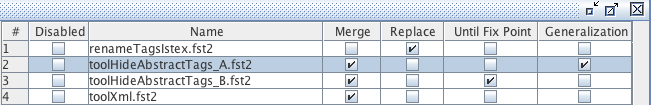
\includegraphics[width=15cm]{resources/img/fig12-3.png}
  \caption{通用图}
  \label{fig12-3}
\end{figure}

\subsection{构造通用图}
在一个通用图的路径必须用\$G和输出,开括号的盒子开始。这是将由CASSYs填充的框。第二个框包含输出要搜索的元素。在\ref{fig12-3-01},在框中输入的每一个类别\textit{x}从文本中提取字典。例如,提取\ EMPH的CASSYs\ textit{A} {\{A,.X\}}字典的文字,如\ref{fig12-3-01a}。此外,负右上下文(section~\ref{section-contexts})放防止第二标签的发生。\begin{figure}[!htb]
  \centering
  \includegraphics[width=5cm]{resources/img/fig12-3-01.png}
  \caption{通用图}
  \label{fig12-3-01}
\end{figure}
\begin{figure}[!htb]
  \centering
  \includegraphics[width=9cm]{resources/img/fig12-3-01a.png}
  \caption{改变通用图}
  \label{fig12-3-01a}
\end{figure}


在\emph{\{\{A,.y\} \{B,.z\},.x\}}参考图\ref{fig12-3-01}发生的情况下,框\textit {AB}如图\ref{fig12-3-02}.

\begin{figure}[!htb]
  \centering
  \includegraphics[width=8cm]{resources/img/fig12-3-02.png}
  \caption{改变通用图}
  \label{fig12-3-02}
\end{figure}

\noindent限制由在第二个框的内部写入类别是可能的,例如:\textit{Y}如图\ref{fig12-3-03};只有\textit{A}这是摆在框中,如图\ref{fig12-3-04}.
\begin{figure}[!htb]
  \centering
  \includegraphics[width=5cm]{resources/img/fig12-3-03.png}
  \caption{带限制的通用图}
  \label{fig12-3-03}
\end{figure}

\begin{figure}[!htb]
  \centering
  \includegraphics[width=8cm]{resources/img/fig12-3-04.png}
  \caption{修改通用图}
  \label{fig12-3-04}
\end{figure}

\bigskip
\bigskip
\bigskip
\bigskip
\bigskip
\bigskip
\bigskip
\bigskip
\noindent相反,一个类别的否定,图例如\textit{\textasciitilde y}中的\ref{fig12-3-05}把\ textit{B}在此框中(figure \ref{fig12-3-06}).
\begin{figure}[!htb]
  \centering
  \includegraphics[width=5cm]{resources/img/fig12-3-05.png}
  \caption{带否定的通用图}
  \label{fig12-3-05}
\end{figure}


\begin{figure}[!htb]
  \centering
  \includegraphics[width=7cm]{resources/img/fig12-3-06.png}
  \caption{修改通用图}
  \label{fig12-3-06}
\end{figure}

如果我们想要补充由一些图不应该寻求的输出,第三框添加为图\ref{fig12-3-07}.
\begin{figure}[!htb]
  \centering
  \includegraphics[width=6cm]{resources/img/fig12-3-07.png}
  \caption{完整的通用图}
  \label{fig12-3-07}
\end{figure}

\section{级联结果}

\subsection{显示级联结果}
\label{subsec:resultsCascade}

级联的应用的结果是一个索引文件(\textit{} concord.ind),如以\textit{"Locate pattern"}一个搜索模式时的情况。该索引文件包含在Unitex控识别的所有序列。

\bigskip
\noindent要查看匹配,只需点击 "Build concordance" 按钮(就像在第\ref{chap-advanced-grammars}章)在"Text / Located sequences"菜单下。 
图\ref{fig13-04}有识别命名实体级联的匹配样本。


\begin{figure}[!htb]
  \centering
  \includegraphics[width=14cm]{resources/img/fig13-04.png}
  \caption{Unitex下的CasSys一致性}
  \label{fig13-04}
\end{figure}

\subsection{级联的各种文件结果}

CasSys保留在级联的每个图形创建的所有文本。这可以是用于测试,调试或从级联不同的结果的验证是有用的。然后就可以纠正错误的图形应用程序的顺序或发现在他们的写作错误。方便的是添加到一个换能器名它的输出,以查看什么原因已经被任何图形识别的最终结果。

如果要应用级联文本example.txt,我们需要创建两个目录:\verb+exemple_snt+ 和\verb+exemple_csc+。
在\verb+exemple_csc+中创建的文件是由每个图得到的结果。这些文件是根据产生它们的曲线图的数目来命名。例如,如果第三个图形识别模式,此图形的应用程序的结果都存储在\verb+exemple_3+\newline\verb+_0_snt+的\verb+exemple_3_0.snt+包括修改后的文本。

\subsection{词法标签的文本XML格式}
文本直接从传感器的应用,并且其中所述词汇标签已被转换为XML的基于XML的格式所得:作为输出,其结果是在两种形式设置。
这种变化是为了提供更可操纵文本到终端用户所作出的。
从这种格式,可以使用的许多XML处理工具之一。
它也很容易,以获得所需的输出,以应用其他出传感器。

文字直接导致换能器存放在文件中 \verb+exemple_csc.raw+, 和XML-isée版本 \verb+exemple_csc.txt+.

具体地说,词汇标签在以下格式~:\\
\begin{tabular}{c}
\texttt{
\{forme.lemme,code1+code2:flex1:flex2\}}
\end{tabular}\\

相应的XML输出格式如下~:\\
\begin{tabular}{ll}
\texttt{<csc>}&\\
    &\texttt{<form>forme</form>}\\
    &\texttt{<lem>lemme</lem>}\\
    &\texttt{<code>code1</code>}\\
    &\texttt{<code>code2</code>}\\
    &\texttt{<inflect>flex1</inflect>}\\
    &\texttt{<inflect>flex2</inflect>}\\
\texttt{</csc>}&\\
\end{tabular}

接下来是DTD的形式:

\begin{tabular}{l}
\texttt{<?xml version="1.0" encoding="ISO-8859-1"?>}\\
\texttt{<!ELEMENT text (\#PCDATA|csc)*>}\\
\texttt{<!ELEMENT csc (form,lem?,code*,inflect*) >}\\
\texttt{<!ELEMENT form (\#PCDATA|csc)*>}\\
\texttt{<!ELEMENT lem (\#PCDATA)>}\\
\texttt{<!ELEMENT code (\#PCDATA)>}\\
\texttt{<!ELEMENT inflect (\#PCDATA)>}\\
\end{tabular}


